\documentclass{article}

% if you need to pass options to natbib, use, e.g.:
%     \PassOptionsToPackage{numbers, compress}{natbib}
% before loading neurips_2021

% ready for submission
\usepackage[preprint]{neurips_2021}
\usepackage{pdfpages}

% to compile a preprint version, e.g., for submission to arXiv, add add the
% [preprint] option:
%     \usepackage[preprint]{neurips_2021}

% to compile a camera-ready version, add the [final] option, e.g.:
%     \usepackage[final]{neurips_2021}

% to avoid loading the natbib package, add option nonatbib:
%    \usepackage[nonatbib]{neurips_2021}

\usepackage[utf8]{inputenc} % allow utf-8 input
\usepackage[T1]{fontenc}    % use 8-bit T1 fonts
\usepackage{hyperref}       % hyperlinks
\usepackage{url}            % simple URL typesetting
\usepackage{booktabs}       % professional-quality tables
\usepackage{amsfonts, bm}       % blackboard math symbols
\usepackage{nicefrac}       % compact symbols for 1/2, etc.
\usepackage{microtype}      % microtypography
\usepackage{xcolor}         % colors
\usepackage{biblatex}       % imports biblatex package

\addbibresource{refs.bib}   % import the bibliography file

\title{Analysing Taxi Data for Traffic Planning and Tourism}

% The \author macro works with any number of authors. There are two commands
% used to separate the names and addresses of multiple authors: \And and \AND.
%
% Using \And between authors leaves it to LaTeX to determine where to break the
% lines. Using \AND forces a line break at that point. So, if LaTeX puts 3 of 4
% authors names on the first line, and the last on the second line, try using
% \AND instead of \And before the third author name.

\author{%
  Wolfgang França Dantas\\
  Matrikelnummer 5717688\\
  \texttt{wolfgang-michael.franca-dantas@} \\
  \texttt{student.uni-tuebingen.de} \\
  \And
  Nils Riekers\\
  Matrikelnummer 5742398\\
  \texttt{nils.riekers@student.uni-tuebingen.de} \\
}
\begin{document}

\maketitle

\begin{center}
\vspace{-1cm}
\url{https://github.com/nilsriekers/data-literacy-project}
\end{center}

\begin{abstract}
We used a collection of New York City taxi trip records \cite{tlc} to identify and visualise popular locations as well as the development of market shares of different types of taxi companies. Furthermore, we wanted to predict how much longer rides take depending on the time of the day in comparison to the shortest possible journey duration. To answer this question, we wanted to use linear regression. However, during our analyses, we found many inconsistencies in the data and the absence of correlations between the destined temporal predictors and the trip duration.
\end{abstract}

\section{Introduction}
As part of the ``Data Literacy'' module, we should gain experience in handling raw data. To do so, we used datasets of taxicab ride records spanning several years from the NYC Taxi and Limousine Commission (TLC). The data itself comes from the ride providers licensed under the Taxicab \& Livery Passenger Enhancement Program. The listed taxi providers are ``Yellow Taxi'', ``Green Taxi'' and ``For-Hire Vehicles'', the latter ones are largely new transportation providers such as Uber or Lyft. The dataset contains information about the individual trips, such as ride time and locations. Our plan was to identify and visualise popular locations. We also wanted to predict how much longer the trips take depending on the time of day compared to the shortest possible trip duration.

\section{Methods}
We established a common standardised workflow in the visualisation and the statistical analysis part to acquire and process our data which consists of the following steps. For each step, we developed separate Python scripts: At first, we procedurally retrieve the taxi data from the official TLC website (\verb|load_taxi_data.py|). After the unification of the data by the loader function, the data directory had a size of about 108 gigabytes. While working with the data, we discovered many inconsistencies which made some pre-processing necessary to remove rows with invalid data like NaN (\verb|preprocess_data.py|), rows with the wrong year (\verb|keep_correct_year.py|), rows with wrong month (\verb|keep_correct_month.py|) and routes that come from or go to locations outside the city (\verb|remove_routes.py|). Afterwards, we extracted temporal features like the month, day, hour and minute of every ride’s pick-up and drop-off as well as the trip duration in minutes (\verb|temporal_preprocessing.py|). As we focused on one particular route, we filtered the trip duration in minutes by introducing a lower (8 minutes) and an upper limit (60 minutes) based on comparisons with average data from Google maps for the chosen route.
For our statistical analyses and the travel time and pick-up visualisations, we limited the data to January 2019.

Additional processing for the statistical analyses: After filtering, we dropped all columns that we would not use any further and only kept \emph{trip\_duration\_minutes}, \emph{pickup\_day\_of\_month}, \emph{pickup\_weekday}, \emph{pickup\_hour}, \emph{pickup\_minute} as final features.

\subsection{Visualisation}
To identify and visualise popular locations, we needed a map of NYC. Fortunately, the TLC provides a shapefile that divides NYC into different cab zones. A shapefile is a simple format for vector geospatial data. All datasets as of 2017 contain data with an indication of the particular pickup and dropout zone of a trip. We used this to visualise data across zones using GeoPandas which is a Python library for extending Pandas objects to support geographic data. For this, we implemented various functions to aggregate the corresponding data across zones.

\subsection{Statistical Analysis}
To investigate correlations between features X and Y, we created correlation matrices using Pearson correlation \(r_{XY}\) as defined in (\ref{pearsonr}). We later ran tests for the significance of the obtained \(r_{XY}\) values using a two-sided test based on the exact distribution of the test statistic which is implemented in SciPy \cite{scipy} (\href{https://docs.scipy.org/doc/scipy/reference/generated/scipy.stats.pearsonr.html}{\texttt{pearsonr}}).
Some data transformations were necessary which we accomplished using simple Box-Cox power transformation (\href{https://docs.scipy.org/doc/scipy/reference/generated/scipy.stats.boxcox.html}{\texttt{boxcox}}, \cite{scipy}) which is defined as (\ref{boxcox})
or Yeo-Johnson power transformation (\href{https://docs.scipy.org/doc/scipy/reference/generated/scipy.stats.yeojohnson.html}{\texttt{yeojohnson}}, \cite{scipy}) which is defined as (\ref{yeojohnson}) in the appendix.

Because of better results in pre-evaluations, we decided for a linear regression model with 3\textsuperscript{rd} degree polynomial basis functions: \(y(\bm{\beta}, \textbf{x}) = \bm\beta^\top\phi(x) \) where \(\phi(x)\) are the basis functions up to degree 3 which include all interactions.

\section{Results \& Discussion}
We restricted the data to focus on one single route from JFK Airport (location ID 132) to LaGuardia Airport (location ID 138) which both are located in Queens (Figure \ref{fig:maps-pickup-travel-time}, left). We made this choice to have a busy route with enough space between the two locations. This was important to make sensible assumptions for filtering the data according to trip duration.

\subsection{Visualisation}
\begin{figure}
  \setlength\abovecaptionskip{-0.3\baselineskip}
  \centering
  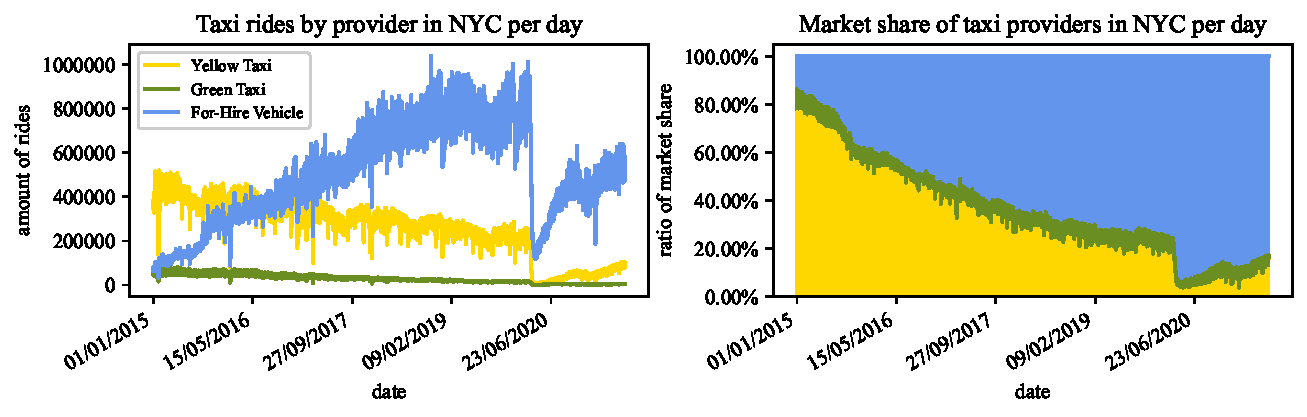
\includegraphics[scale=0.63]{fig/taxi-rides-over-time.pdf}
  \caption{Taxi rides by provider and provider market share in NYC per day.}
  \label{fig:taxi-rides-over-time}
\end{figure}
\setlength{\textfloatsep}{10pt}
Figure \ref{fig:taxi-rides-over-time} shows on its left half the number of daily taxi trips in NYC in the period from January 2015 to the end of June 2021 visualised by a line plot. On its right side, Figure 1 shows the ratio of market share among the taxi providers in the same period visualised by an area plot. It can be seen very clearly that the provider Yellow-Taxi performed continuously fewer trips over time. Meanwhile, the providers of the For-Hire Vehicles have steadily operated an increasing number of trips since the beginning of 2015. The providers of the For-Hire Vehicles took the market leadership of the taxi market in NYC in the first half of 2017, replacing Yellow-Taxi. The rides and as well as the market share of the provider Green Taxi was permanently at a low, but relatively constant level. In the beginning of 2020, we see a very sharp drop in the amount of daily rides. This was caused by the lockdown due to the Corona virus. By the end of June 2021, the transport volume of all taxi providers had not recovered. With the beginning of the first lockdown, the market leadership of the For-Hire Vehicles providers has further increased. The increasing digitalization is probably the reason why the new providers of the for-hire vehicles, such as Uber or Lyft, are replacing the traditional enterprises.
\begin{figure}
  \setlength\abovecaptionskip{-0.3\baselineskip}
  \centering
  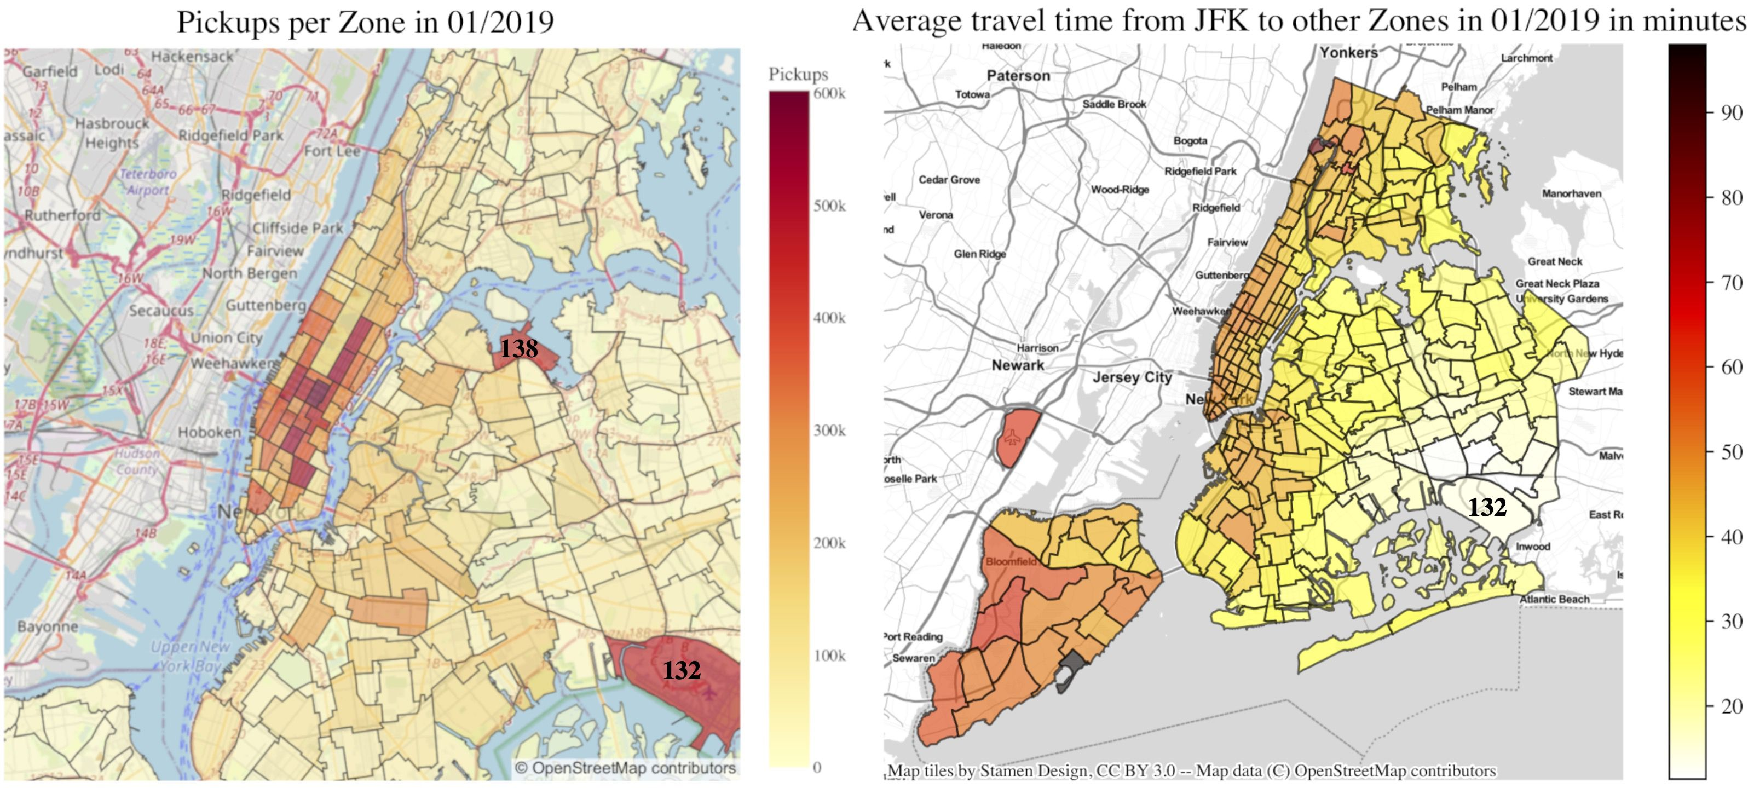
\includegraphics[scale=0.47]{fig/maps-pickup-travel-time.pdf}
  \caption{Pickups per Zone and average travel time from JFK to other Zones in 01/2019.}
  \label{fig:maps-pickup-travel-time}
\end{figure}
\setlength{\textfloatsep}{10pt}

Figure \ref{fig:maps-pickup-travel-time} shows on its left half the number of cab pickups in NYC per zone in January 2019 visualized by a heat map. In brighter zones, fewer pickups took place, while in red zones there were more. The zone with the ID 132, the John F. Kennedy Airport (JFK), as well as the zone with the ID 138, the LaGuardia Airport (LGA), were manually supplemented with a number to mark them. It can be seen that especially the downtown area in Manhattan, as well as the two airports JFK and LGA were highly frequented places for pickups of taxi rides. This is probably due to the fact that in Manhattan, compared to the other parts of the city, an above-average number of people work, live and also visit for tourist purposes. The high number of pickups at the airports is probably due to a high volume of travellers. On its right side, Figure \ref{fig:maps-pickup-travel-time} shows the average travel time in minutes from the JFK airport with ID 132 to the other zones.
\begin{figure}
  \vspace{-0.5cm}
  \setlength\abovecaptionskip{-0.3\baselineskip}
  \centering
  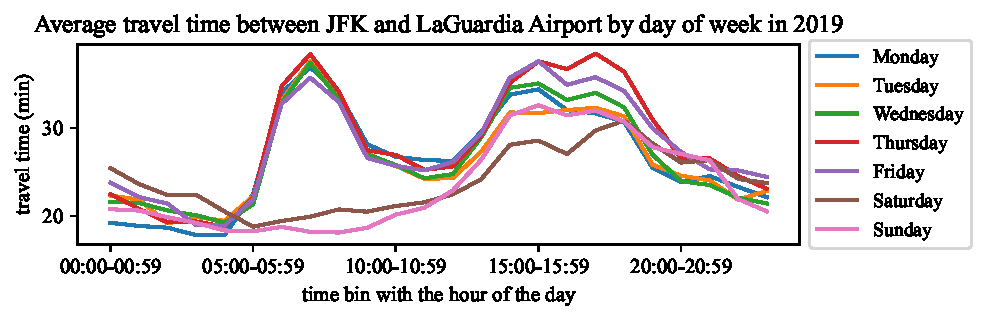
\includegraphics[scale=0.70]{fig/travel-time-from-JFK-to-LGA.pdf}
  \caption{Average travel time between JFK and LaGuardia Airport by day of week in 2019.}
  \label{fig:travel-time-from-JFK-to-LGA}
\end{figure}
\setlength{\textfloatsep}{10pt}

It gets more interesting looking at Figure \ref{fig:travel-time-from-JFK-to-LGA}, it shows the average travel time between JFK and LaGuardia Airport by day of the week throughout 2019 in a line graph. It is clear to see that there are different rush hours, where the travel time is much longer than at other times. Thus, there is a peak between 7 and 9 am and a peak between 2 and 7 pm. However, on the weekend days of Saturday and Sunday, this peak is absent in the morning and less intense in the afternoon. This suggests that these times are most likely due to commuting.

\subsection{Statistical Analysis}

\begin{figure}
  \setlength\abovecaptionskip{-0.3\baselineskip}
  \centering
  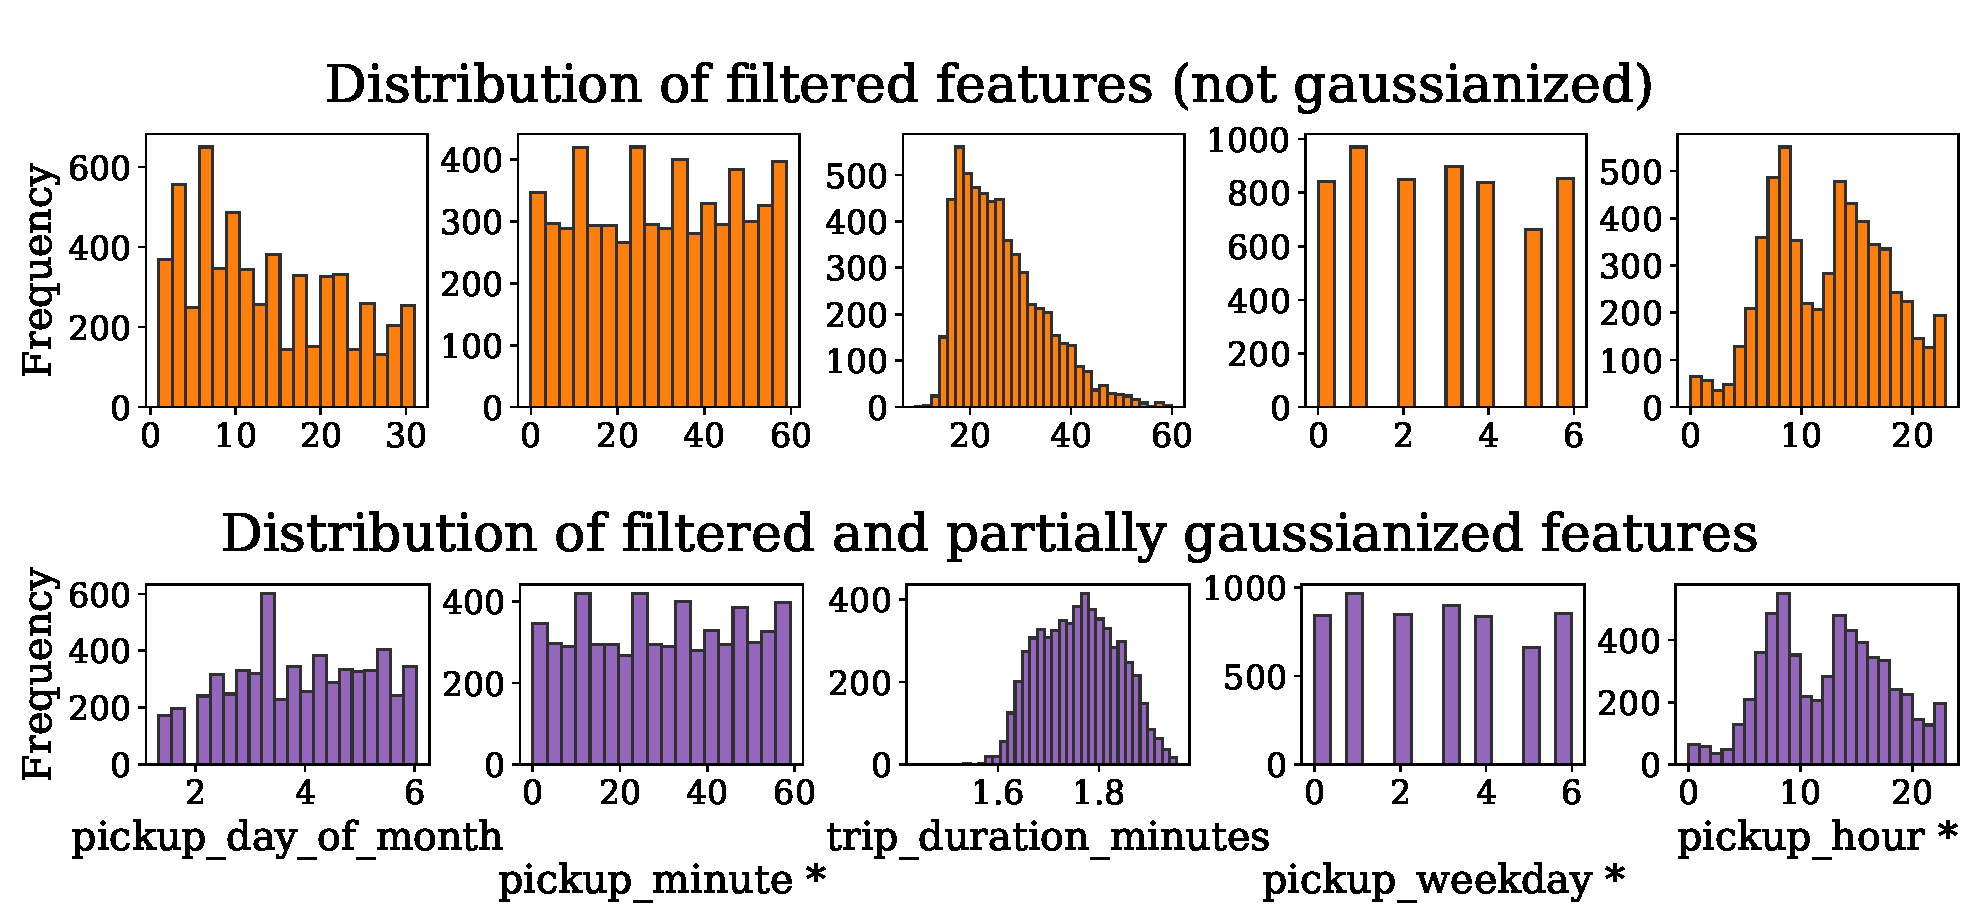
\includegraphics[scale=0.38]{fig/feature_distributions.pdf}
  \caption{Distribution of features before and after partial gaussianization. Route from location ID 132 to ID 138 in 01/2019. * indicates that gaussianization was not possible with simple transformations.}
  \label{fig:feature_distributions}
\end{figure}
\begin{figure}
  \setlength\abovecaptionskip{-0.3\baselineskip}
  \centering
  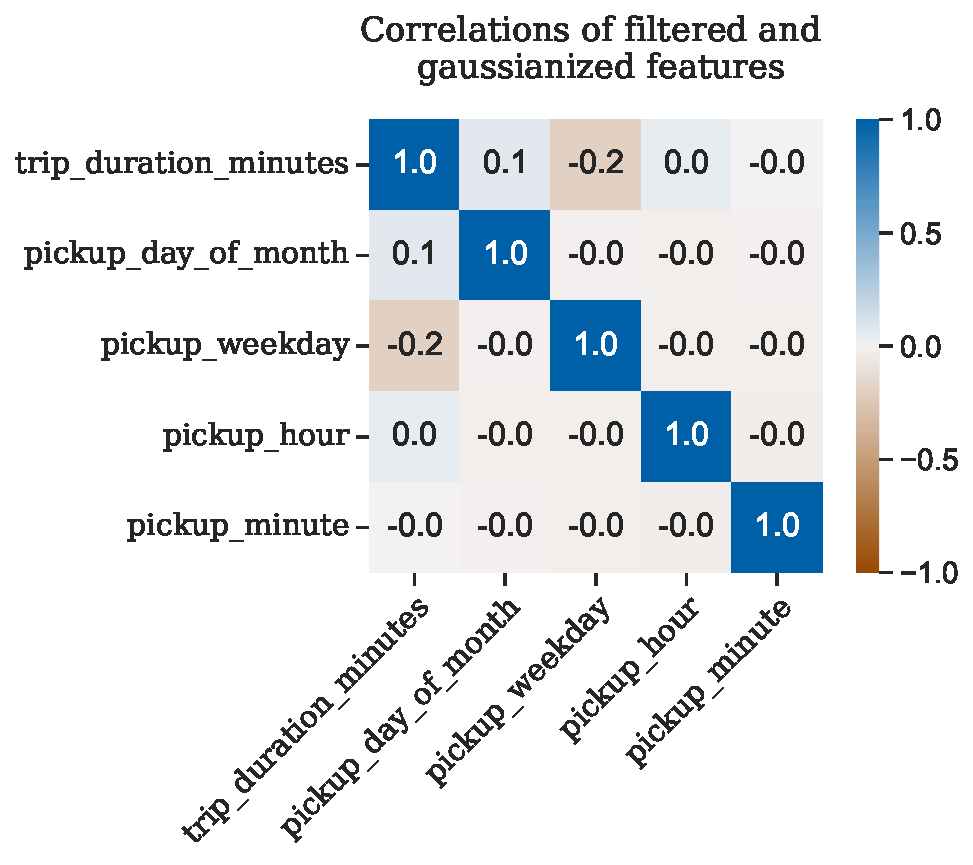
\includegraphics[scale=0.45]{fig/correlations_gaussianized_columns_route_132_138.pdf}
  \caption{Correlations of filtered and partially gaussianized features. Route from location ID 132 to ID 138 in 01/2019.}
  \label{fig:correlation_matrix}
\end{figure}

After filtering the data, we wanted to analyse Pearson correlations between features to select the best predictors for our regression model. However, we found that the data was not Gaussian at all (Figure \ref{fig:feature_distributions} top). This is problematic as Gaussian data is a prerequisite to the Pearson correlation. Therefore, we tried to ``gaussianize'' the data using non-linear yet simple Box-Cox and Yeo-Johnson transformations which were only partially successful (Figure \ref{fig:feature_distributions} bottom). We are aware that this criterion, thus, is violated and the correlation coefficients shown in Figure \ref{fig:correlation_matrix} may only have limited validity.

Based on these results, we tested the significance of the correlations between \emph{trip\_duration\_minutes} \(\times\) \emph{pickup\_weekday} (\(r = -0.19\), \(p<0.0001\)), \emph{trip\_duration\_minutes} \(\times\) \emph{pickup\_day\_of\_month} (\(r = 0.06\), \(p<0.0001\)), \emph{trip\_duration\_minutes} \(\times\) \emph{pickup\_hour} (\(r = 0.04\), \(p= 0.0011\)) and \emph{trip\_duration\_minutes} \(\times\) \emph{pickup\_minute} (\(r = -0.01\), \(p=0.6853\)).
Finally, we divided our entire filtered data (5912 rows) into training and test set (\(10\%\) of the entire data set) and fitted a linear regression model with 3\textsuperscript{rd} order polynomial basis functions to the data whose coefficient of determination evaluated to \(\textrm{R}^2=0.2\).

In cases where \(r_{XY} \approx 0\), this indicates that there is no correlation between the trip duration in minutes and the respective feature. From the highly significant p-values from the two-sided test for correlation we conclude that there actually is no correlation. The \(r_{XY}\) value obtained is too unlikely to having occurred by chance. Despite a non-significant p-value of the \emph{trip\_duration\_minutes} \(\times\) \emph{pickup\_minute} correlation, we still assume no correlation due to the violated criterion of Gaussianity. Assuming no correlations, all variables are stochastically linearly independent. This explains why the linear regression could not work with the target-feature combinations we initially chose and also is reflected by the small R\textsuperscript{2} value. From Figure \ref{fig:travel-time-from-JFK-to-LGA}  we rather would conclude highly non-linear relationships. Thus, the basis functions we used were too simple to capture them.

\section{Overall conclusion}
In conclusion, we found that lots of care has to be taken when using this data set. Inconsistent and implausible data can, when not discovered, distort the results of possible analyses. Many decisions have to be taken by the user of the data how to filter it and how to extract the sensible bits as little documentation is provided by the TLC \cite{tlc} about how the data is generated. Furthermore, linear regression based on temporal features is not possible due to their non-linear nature.

\printbibliography % Prints bibliography

\appendix
\section{Appendix}
Formulas mentioned in the methods section:

\begin{equation}\label{pearsonr}
    r_{YX} = \frac{\sum (x-\bar{x})(y-\bar{y})}{\sqrt{\sum (x-\bar{x})^2 \sum (y-\bar{y})^2}}
\end{equation}

\vspace{5mm} %5mm vertical space

\begin{equation}\label{boxcox}
         \widetilde{x}_{BC}(x)=\left\{\begin{array}{ll} \frac{x^\lambda - 1}{\lambda}, & \lambda \neq 0 \\ \\
         log(x), & \lambda = 0\end{array}\right.
\end{equation}

\vspace{5mm} %5mm vertical space

\begin{equation}\label{yeojohnson}
         \widetilde{x}_{YJ}(x)=\left\{\begin{array}{ll} \frac{(x+1)^\lambda -1}{\lambda}, & x \geq 0 \; \textrm{and} \;  \lambda \neq 0 \\ \\
         log(x+1), & x \geq 0 \; \textrm{and} \; \lambda = 0 \\ \\
         -\frac{(-x+1)^{2-\lambda}-1}{2-\lambda}, & x < 0 \; \textrm{and} \; \lambda \neq 2 \\ \\
         -log(-x+1), & x < 0 \; \textrm{and} \; \lambda = 2\end{array} \right.
\end{equation}

\end{document}
